\section{Methodology}

In this section, I will detail the analysis methods used in my research, including model selection, parameter settings, and validation strategies.

To begin, I conducted a train-test split on the dataset, where I divided the data into training and testing sets with a ratio of 80:20. 
This split was chosen to ensure that there is a substantial amount of data for training the models while retaining a sufficient portion for testing their generalization capabilities. 
An 80:20 split is a common practice in machine learning, providing a good balance between training performance and validation accuracy. By allocating 80\% of the data for training, 
the models can be adequately trained capture the underlying patterns in the data. The remaining 20\% serves as an unbiased test set to evaluate the models performance on unseen data.

\subsection{Machine Learning Methodology}

To evaluate the models performances, I used a 5-fold cross-validation strategy using "StratifiedKFold", ensuring that each fold preserves the percentage of samples for each class. 
This method enhances the reliability of performance estimates by mitigating the variance associated with a single train-test split. Cross-validation provides multiple performance 
estimates, which gives a better understanding of how the models will perform in practice. The choice of 5 folds strikes a balance between bias and variance: while more folds can 
provide better estimates, they also require more computational resources and can lead to longer training times. The metrics evaluated during cross-validation included accuracy, 
F1 score, recall, and precision.

For this part of the research, I experimented with two distinct text representation techniques: Term Frequency-Inverse Document Frequency (TF-IDF) and Bag of Words (BoW). 
For the TF-IDF vectorization, I utilized the TfidfVectorizer, configuring it to extract n-grams ranging from unigrams to trigrams while limiting the maximum number of features to 50,000. 
This configuration was chosen to capture both individual words and phrases that may convey sarcasm, allowing the model to leverage contextual information effectively. 
Similarly, for the BoW representation, I used CountVectorizer with the same n-gram range and feature limit. Both representations enable the models to learn from the frequency of terms, 
helping them identify patterns indicative of sarcasm.

I tested four machine learning models: Logistic Regression and Ridge Classifier, each applied to both TF-IDF and BoW representations. The Logistic Regression model was configured with 
a regularization parameter "C" set to 0.5 and L2 penalty, while the Ridge Classifier was set with an alpha parameter of 1.0. The choice of "C" was based on prior research indicating that 
moderate regularization often yields better performance in text classification tasks by preventing overfitting. The L2 penalty further enhances model generalization by constraining the 
coefficients. For the Ridge Classifier, the alpha parameter of 1.0 was selected to provide a strong regularization effect while still allowing the model to capture significant features 
in the data, ensuring balanced performance.

After evaluating the models, I calculated the mean and standard deviation of the metrics across the folds to provide an assessment of each model's performance. This approach not only 
helps in identifying the best-performing model but also in understanding the stability and reliability of the results. Additionally, I generated confusion matrices to visualize each 
model's classification results, which aids in understanding misclassifications and the distribution of true positives, false positives, true negatives, and false negatives. 
The best model, according to mainly to accuracy or other metrics in case of an equality, will be trained on the full dataset.

\subsection{Deep Learning Methodology}

For the deep learning component of this research, I implemented models based on Long Short-Term Memory (LSTM) networks, utilizing two types of pre-trained word embeddings: 
GloVe and Word2Vec.

I began by tokenizing the input text data using TensorFlow's Tokenizer. This involved converting the text comments into sequences of integers, where each integer represents a specific 
word in the dataset. The tokenizer was configured to retain the 40,000 most frequent words, ensuring that the model could learn from a rich vocabulary while minimizing noise from 
infrequent terms. The resulting sequences were then padded to a maximum length of 100 tokens. This padding helps to standardize input dimensions across different samples, which is 
crucial for LSTM networks that require consistent input shapes.

To represent the textual data in a way that captures semantic meaning, I employed two popular pre-trained word embedding techniques: GloVe and Word2Vec. 

For GloVe, I downloaded the pre-trained embeddings and constructed an embedding matrix that maps each word in the vocabulary to its corresponding GloVe vector. 
The embeddings were set to 50 dimensions, balancing representational capacity with computational efficiency. I chose to keep the embeddings non-trainable during model training to 
leverage the general knowledge captured in the pre-trained vectors, which has been shown to enhance performance in text classification tasks.

Similarly, for the Word2Vec embeddings, I trained a Word2Vec model on the tokenized training data. The embedding dimension was also set to 50, and the window size was configured to 5, 
which allows the model to capture context within that range. This embedding captures relationships between words based on their co-occurrence in the training data.

The core of my deep learning model consisted of a single-layer LSTM architecture.
Given the large dataset of over one million rows, the architecture is intentionally kept simple to balance computational efficiency and model performance. 
The LSTM model layer architecture is displayed in Figure \ref{Fig_3}.

\begin{figure}
    \centering
    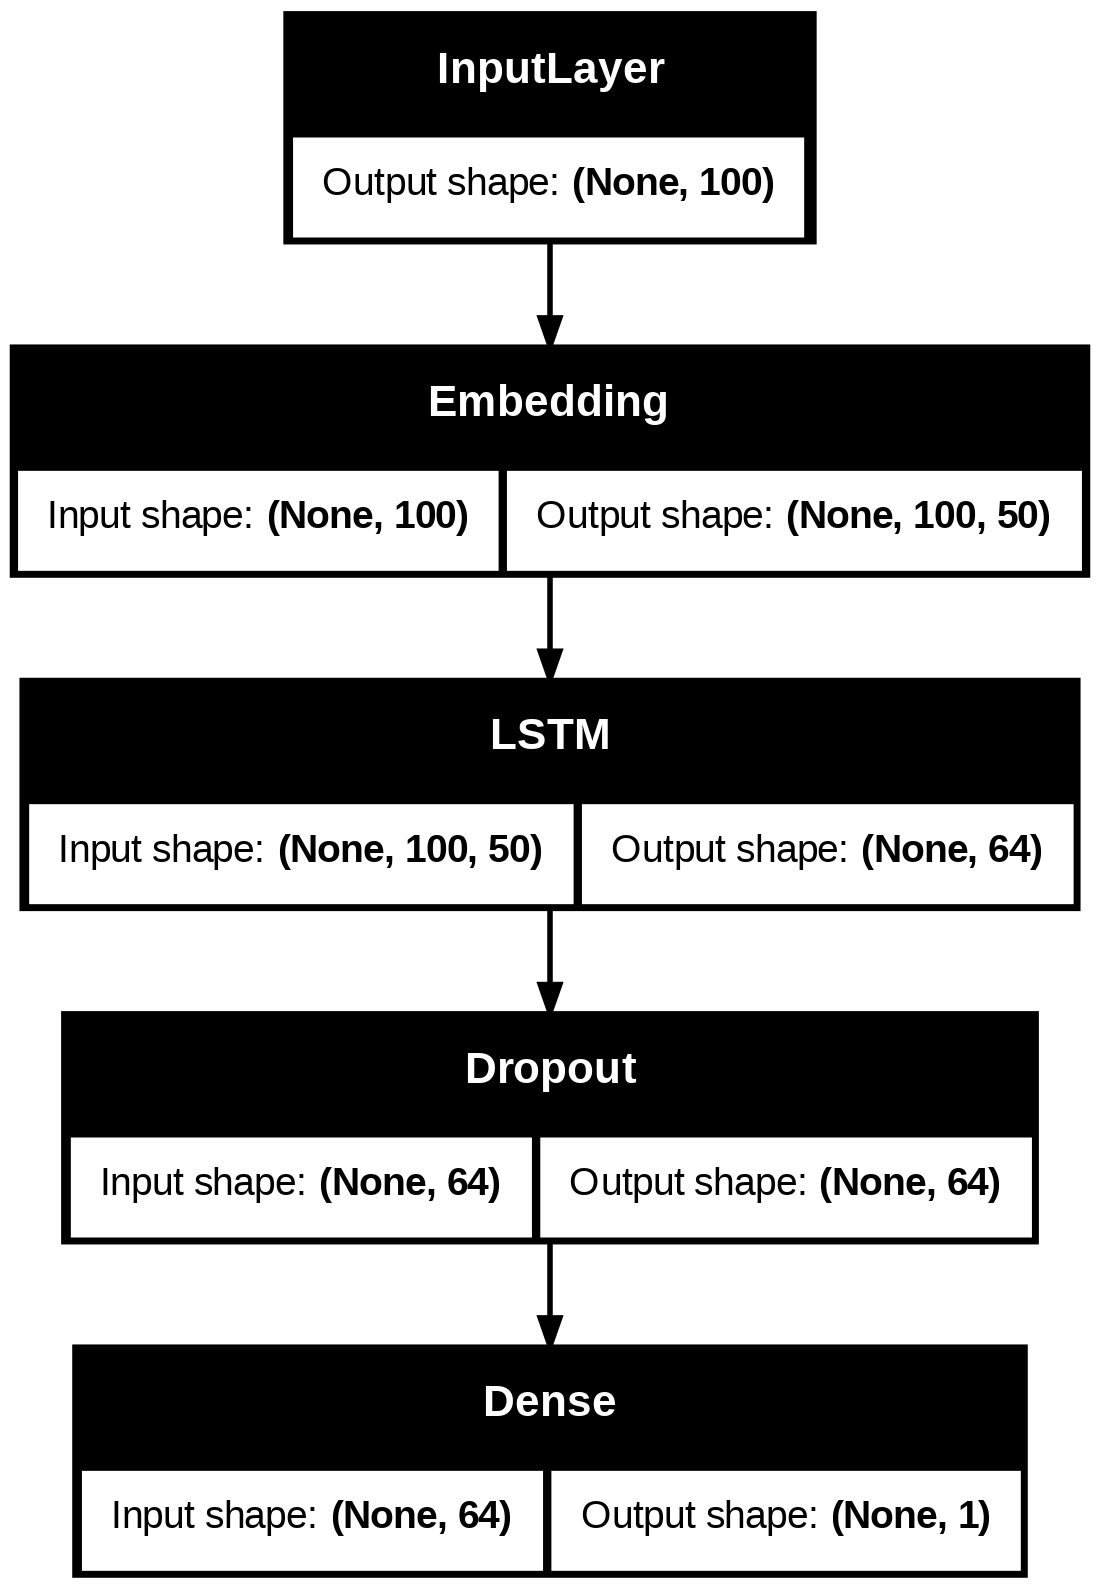
\includegraphics[width=0.5\linewidth]{img/model-layers.png}
    \caption{LSTM Model Layer Architecture}
    \label{Fig_3}
\end{figure}

The model begins with an Input Layer, where the max length is set to 100. This layer specifies the expected shape of the input of 100 tokens per example. 
The "None" in the shape represents the batch size, determined during training. This layer itself does not perform any computation but acts as a placeholder to feed data into the network.

Next, the Embedding Layer transforms input word indices into dense vector representations. This layer converts each word into a vector of size 50. The weights argument allows for the 
use of a pre-trained word embedding matrix, such as GloVe or Word2Vec, leveraging prior linguistic knowledge. By setting the trainable parameter to "False", the pre-trained embeddings 
remain static during training, reducing computational cost and preventing overfitting. The output shape of this layer is (None, 100, 50), indicating a sequence of 100 words, each 
represented by a 50-dimensional vector.

Following the embedding, the LSTM Layer captures temporal relationships in the input sequence. It processes the 100-word sequence and outputs a 64-dimensional vector representing the 
final hidden state. Here, the parameter "return sequences" is set to "False" to ensure only the last hidden state is passed to the next layer.

To prevent overfitting, the model incorporates a Dropout Layer. This layer randomly sets 50{\%} of the neurons to zero during training, ensuring the model does not overly rely on 
specific features. Dropout is a widely used regularization technique, particularly effective when dealing with large datasets.

The final prediction is made by a Dense Layer. This fully connected layer has a single neuron with a sigmoid activation function, outputting a probability between 0 and 1. 
This probability represents the likelihood that the input text is sarcastic. A value closer to 1 suggests sarcasm, while a value near 0 indicates non-sarcastic content.

The model is compiled using the binary cross-entropy loss function, suitable for binary classification tasks. I chose "adam" as the optimizer because it combines the benefits of momentum
and "RMSprop". The accuracy metric evaluates model performance by comparing predicted labels with true labels.

The models were trained using a validation split of 20\% from the training data to monitor performance and prevent overfitting. The training process employed early stopping, monitoring 
validation accuracy with a patience of 3 epochs. This means that if the validation accuracy did not improve for three consecutive epochs, the training would halt, and the best model 
weights would be restored. The batch size was set to 1024, which allows for efficient use of GPU resources, and the model was trained for a maximum of 20 epochs. The training duration
was managed to avoid overfitting while ensuring adequate learning.

Once trained, I evaluated the performance of each model on the test set using metrics such as accuracy, precision, recall, and F1 score. These metrics provided a comprehensive assessment
of the model's ability to detect sarcasm in unseen data.